\documentclass[twoside]{book}

% Packages required by doxygen
\usepackage{fixltx2e}
\usepackage{calc}
\usepackage{doxygen}
\usepackage{graphicx}
\usepackage[utf8]{inputenc}
\usepackage{makeidx}
\usepackage{multicol}
\usepackage{multirow}
\PassOptionsToPackage{warn}{textcomp}
\usepackage{textcomp}
\usepackage[nointegrals]{wasysym}
\usepackage[table]{xcolor}

% Font selection
\usepackage[T1]{fontenc}
\usepackage{mathptmx}
\usepackage[scaled=.90]{helvet}
\usepackage{courier}
\usepackage{amssymb}
\usepackage{sectsty}
\renewcommand{\familydefault}{\sfdefault}
\allsectionsfont{%
  \fontseries{bc}\selectfont%
  \color{darkgray}%
}
\renewcommand{\DoxyLabelFont}{%
  \fontseries{bc}\selectfont%
  \color{darkgray}%
}
\newcommand{\+}{\discretionary{\mbox{\scriptsize$\hookleftarrow$}}{}{}}

% Page & text layout
\usepackage{geometry}
\geometry{%
  a4paper,%
  top=2.5cm,%
  bottom=2.5cm,%
  left=2.5cm,%
  right=2.5cm%
}
\tolerance=750
\hfuzz=15pt
\hbadness=750
\setlength{\emergencystretch}{15pt}
\setlength{\parindent}{0cm}
\setlength{\parskip}{0.2cm}
\makeatletter
\renewcommand{\paragraph}{%
  \@startsection{paragraph}{4}{0ex}{-1.0ex}{1.0ex}{%
    \normalfont\normalsize\bfseries\SS@parafont%
  }%
}
\renewcommand{\subparagraph}{%
  \@startsection{subparagraph}{5}{0ex}{-1.0ex}{1.0ex}{%
    \normalfont\normalsize\bfseries\SS@subparafont%
  }%
}
\makeatother

% Headers & footers
\usepackage{fancyhdr}
\pagestyle{fancyplain}
\fancyhead[LE]{\fancyplain{}{\bfseries\thepage}}
\fancyhead[CE]{\fancyplain{}{}}
\fancyhead[RE]{\fancyplain{}{\bfseries\leftmark}}
\fancyhead[LO]{\fancyplain{}{\bfseries\rightmark}}
\fancyhead[CO]{\fancyplain{}{}}
\fancyhead[RO]{\fancyplain{}{\bfseries\thepage}}
\fancyfoot[LE]{\fancyplain{}{}}
\fancyfoot[CE]{\fancyplain{}{}}
\fancyfoot[RE]{\fancyplain{}{\bfseries\scriptsize Generated on Wed Jul 27 2016 20\+:05\+:35 for nethorn by Doxygen }}
\fancyfoot[LO]{\fancyplain{}{\bfseries\scriptsize Generated on Wed Jul 27 2016 20\+:05\+:35 for nethorn by Doxygen }}
\fancyfoot[CO]{\fancyplain{}{}}
\fancyfoot[RO]{\fancyplain{}{}}
\renewcommand{\footrulewidth}{0.4pt}
\renewcommand{\chaptermark}[1]{%
  \markboth{#1}{}%
}
\renewcommand{\sectionmark}[1]{%
  \markright{\thesection\ #1}%
}

% Indices & bibliography
\usepackage{natbib}
\usepackage[titles]{tocloft}
\setcounter{tocdepth}{3}
\setcounter{secnumdepth}{5}
\makeindex

% Hyperlinks (required, but should be loaded last)
\usepackage{ifpdf}
\ifpdf
  \usepackage[pdftex,pagebackref=true]{hyperref}
\else
  \usepackage[ps2pdf,pagebackref=true]{hyperref}
\fi
\hypersetup{%
  colorlinks=true,%
  linkcolor=blue,%
  citecolor=blue,%
  unicode%
}

% Custom commands
\newcommand{\clearemptydoublepage}{%
  \newpage{\pagestyle{empty}\cleardoublepage}%
}


%===== C O N T E N T S =====

\begin{document}

% Titlepage & ToC
\hypersetup{pageanchor=false,
             bookmarks=true,
             bookmarksnumbered=true,
             pdfencoding=unicode
            }
\pagenumbering{roman}
\begin{titlepage}
\vspace*{7cm}
\begin{center}%
{\Large nethorn }\\
\vspace*{1cm}
{\large Generated by Doxygen 1.8.8}\\
\vspace*{0.5cm}
{\small Wed Jul 27 2016 20:05:35}\\
\end{center}
\end{titlepage}
\clearemptydoublepage
\tableofcontents
\clearemptydoublepage
\pagenumbering{arabic}
\hypersetup{pageanchor=true}

%--- Begin generated contents ---
\chapter{nethorn}
\label{md__r_e_a_d_m_e}
\hypertarget{md__r_e_a_d_m_e}{}
A C++11 library to generate (raw) packets and manage low-\/level sessions by hand. 
\chapter{Class Index}
\section{Class List}
Here are the classes, structs, unions and interfaces with brief descriptions\+:\begin{DoxyCompactList}
\item\contentsline{section}{\hyperlink{class_n_h_1_1_protocols_1_1_raw_1_1ethernet__t}{N\+H\+::\+Protocols\+::\+Raw\+::ethernet\+\_\+t} \\*Ethernet\+\_\+t Is a class that helps generating ethernet frames }{\pageref{class_n_h_1_1_protocols_1_1_raw_1_1ethernet__t}}{}
\item\contentsline{section}{\hyperlink{classethernet__t}{ethernet\+\_\+t} \\*Constructs Constructs object using raw {\ttfamily \+\_\+data\+\_\+a} ethernet data with {\ttfamily \+\_\+size\+\_\+a} size }{\pageref{classethernet__t}}{}
\item\contentsline{section}{\hyperlink{classethernet__t}{ethernet\+\_\+t} \\*Default constructor }{\pageref{classethernet__t}}{}
\item\contentsline{section}{\hyperlink{classexception__t}{exception\+\_\+t} \\*Sets source M\+A\+C address }{\pageref{classexception__t}}{}
\item\contentsline{section}{\hyperlink{classexception__t}{exception\+\_\+t} \\*Erases given pot region }{\pageref{classexception__t}}{}
\item\contentsline{section}{\hyperlink{classexception__t}{exception\+\_\+t} }{\pageref{classexception__t}}{}
\item\contentsline{section}{\hyperlink{classexception__t}{exception\+\_\+t} \\*Activates the 802.\+1\+Q extension }{\pageref{classexception__t}}{}
\item\contentsline{section}{\hyperlink{classexception__t}{exception\+\_\+t} \\*Sets destination M\+A\+C address }{\pageref{classexception__t}}{}
\item\contentsline{section}{\hyperlink{class_n_h_1_1_protocols_1_1_raw_1_1pot__t}{N\+H\+::\+Protocols\+::\+Raw\+::pot\+\_\+t} \\*Pot\+\_\+t Is a class that allows manipulation over raw data }{\pageref{class_n_h_1_1_protocols_1_1_raw_1_1pot__t}}{}
\end{DoxyCompactList}

\chapter{Class Documentation}
\hypertarget{class_n_h_1_1_protocols_1_1_raw_1_1_ethernet}{\section{N\+H\+:\+:Protocols\+:\+:Raw\+:\+:Ethernet Class Reference}
\label{class_n_h_1_1_protocols_1_1_raw_1_1_ethernet}\index{N\+H\+::\+Protocols\+::\+Raw\+::\+Ethernet@{N\+H\+::\+Protocols\+::\+Raw\+::\+Ethernet}}
}


The documentation for this class was generated from the following file\+:\begin{DoxyCompactItemize}
\item 
include/protocols/raw/eth.\+hxx\end{DoxyCompactItemize}

\hypertarget{class_n_h_1_1_protocols_1_1_raw_1_1pot__t}{\section{N\+H\+:\+:Protocols\+:\+:Raw\+:\+:pot\+\_\+t Class Reference}
\label{class_n_h_1_1_protocols_1_1_raw_1_1pot__t}\index{N\+H\+::\+Protocols\+::\+Raw\+::pot\+\_\+t@{N\+H\+::\+Protocols\+::\+Raw\+::pot\+\_\+t}}
}


\hyperlink{class_n_h_1_1_protocols_1_1_raw_1_1pot__t}{pot\+\_\+t} Is a class that allows manipulation over raw data.  




{\ttfamily \#include $<$pot.\+hxx$>$}

Inheritance diagram for N\+H\+:\+:Protocols\+:\+:Raw\+:\+:pot\+\_\+t\+:\begin{figure}[H]
\begin{center}
\leavevmode
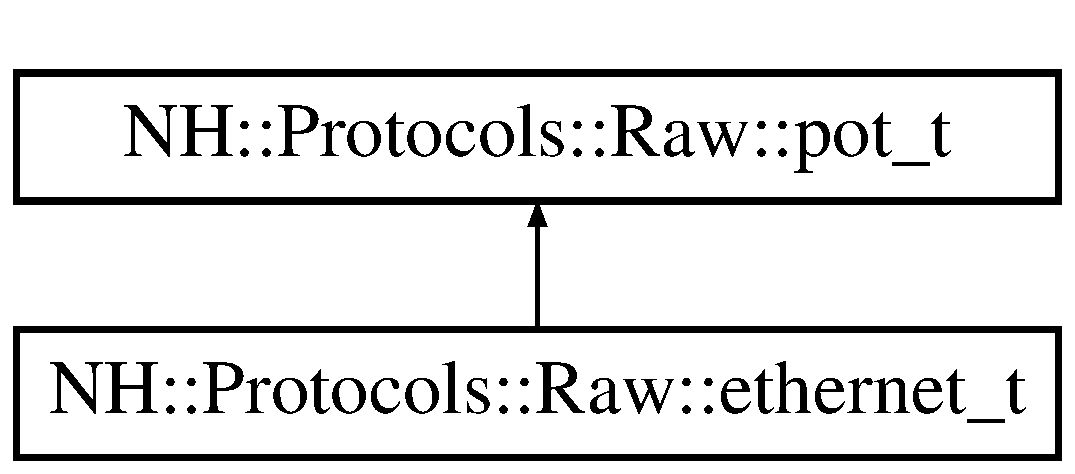
\includegraphics[height=2.000000cm]{class_n_h_1_1_protocols_1_1_raw_1_1pot__t}
\end{center}
\end{figure}
\subsection*{Public Member Functions}
\begin{DoxyCompactItemize}
\item 
\hyperlink{class_n_h_1_1_protocols_1_1_raw_1_1pot__t_af086f3f10e88f3f906a0fd5c9901d4f1}{pot\+\_\+t} () noexcept
\begin{DoxyCompactList}\small\item\em Default constructor. \end{DoxyCompactList}\item 
\hyperlink{class_n_h_1_1_protocols_1_1_raw_1_1pot__t_a4c2c3964a61735786ec9e31b10524f7c}{pot\+\_\+t} (const uint8\+\_\+t $\ast$\+\_\+data\+\_\+a, uint32\+\_\+t \+\_\+size\+\_\+a)  throw (exception\+\_\+t)
\begin{DoxyCompactList}\small\item\em Non-\/default constructor. \end{DoxyCompactList}\item 
\hyperlink{class_n_h_1_1_protocols_1_1_raw_1_1pot__t_ae40dc98cefa4754adcd154928f5d6fe3}{pot\+\_\+t} (uint32\+\_\+t \+\_\+size\+\_\+a)  throw (exception\+\_\+t)
\begin{DoxyCompactList}\small\item\em Non-\/default constructor. \end{DoxyCompactList}\item 
\hypertarget{class_n_h_1_1_protocols_1_1_raw_1_1pot__t_a378d13cc9b400920d62cbc0edcbd08ef}{\hyperlink{class_n_h_1_1_protocols_1_1_raw_1_1pot__t_a378d13cc9b400920d62cbc0edcbd08ef}{pot\+\_\+t} (const \hyperlink{class_n_h_1_1_protocols_1_1_raw_1_1pot__t}{pot\+\_\+t} \&\+\_\+pot\+\_\+a) noexcept}\label{class_n_h_1_1_protocols_1_1_raw_1_1pot__t_a378d13cc9b400920d62cbc0edcbd08ef}

\begin{DoxyCompactList}\small\item\em Copy constructor. \end{DoxyCompactList}\item 
\hypertarget{class_n_h_1_1_protocols_1_1_raw_1_1pot__t_aadc3a3bd8e3d337b9c9cbde868cfb047}{\hyperlink{class_n_h_1_1_protocols_1_1_raw_1_1pot__t_aadc3a3bd8e3d337b9c9cbde868cfb047}{pot\+\_\+t} (\hyperlink{class_n_h_1_1_protocols_1_1_raw_1_1pot__t}{pot\+\_\+t} \&\&\+\_\+pot\+\_\+a) noexcept}\label{class_n_h_1_1_protocols_1_1_raw_1_1pot__t_aadc3a3bd8e3d337b9c9cbde868cfb047}

\begin{DoxyCompactList}\small\item\em Move constructor. \end{DoxyCompactList}\item 
\hypertarget{class_n_h_1_1_protocols_1_1_raw_1_1pot__t_a6dff7ad396d312de62f1a4568b4ec51c}{virtual \hyperlink{class_n_h_1_1_protocols_1_1_raw_1_1pot__t_a6dff7ad396d312de62f1a4568b4ec51c}{$\sim$pot\+\_\+t} () noexcept}\label{class_n_h_1_1_protocols_1_1_raw_1_1pot__t_a6dff7ad396d312de62f1a4568b4ec51c}

\begin{DoxyCompactList}\small\item\em Destructor. \end{DoxyCompactList}\item 
const \hyperlink{class_n_h_1_1_protocols_1_1_raw_1_1pot__t}{pot\+\_\+t} \& \hyperlink{class_n_h_1_1_protocols_1_1_raw_1_1pot__t_a65d782c7d72c93a090f3ae24215fb1bb}{operator=} (const \hyperlink{class_n_h_1_1_protocols_1_1_raw_1_1pot__t}{pot\+\_\+t} \&\+\_\+pot\+\_\+a) noexcept
\begin{DoxyCompactList}\small\item\em Assign operator. \end{DoxyCompactList}\item 
const \hyperlink{class_n_h_1_1_protocols_1_1_raw_1_1pot__t}{pot\+\_\+t} \& \hyperlink{class_n_h_1_1_protocols_1_1_raw_1_1pot__t_a17dfa779637feb4361afd41379ee29a4}{operator=} (\hyperlink{class_n_h_1_1_protocols_1_1_raw_1_1pot__t}{pot\+\_\+t} \&\&\+\_\+pot\+\_\+a) noexcept
\begin{DoxyCompactList}\small\item\em Move operator. \end{DoxyCompactList}\item 
const uint8\+\_\+t $\ast$ \hyperlink{class_n_h_1_1_protocols_1_1_raw_1_1pot__t_af67504820aeff86c904925983d4644a1}{data} () const noexcept
\begin{DoxyCompactList}\small\item\em Returns pot. \end{DoxyCompactList}\item 
uint8\+\_\+t \hyperlink{class_n_h_1_1_protocols_1_1_raw_1_1pot__t_aebfc8267a6c20674a4cf7a2cd00081be}{operator\mbox{[}$\,$\mbox{]}} (int32\+\_\+t \+\_\+index\+\_\+a) const   throw (exception\+\_\+t)
\begin{DoxyCompactList}\small\item\em Accesses pot by {\ttfamily \+\_\+index\+\_\+a} index. \end{DoxyCompactList}\item 
uint8\+\_\+t \& \hyperlink{class_n_h_1_1_protocols_1_1_raw_1_1pot__t_a407f77712662868c1646f1a7c44e545a}{operator\mbox{[}$\,$\mbox{]}} (int32\+\_\+t \+\_\+index\+\_\+a)  throw (exception\+\_\+t)
\begin{DoxyCompactList}\small\item\em Accesses pot by {\ttfamily \+\_\+index\+\_\+a} index. \end{DoxyCompactList}\item 
uint32\+\_\+t \hyperlink{class_n_h_1_1_protocols_1_1_raw_1_1pot__t_a57a62cf7952f487a5ef513fabc2cdeed}{size} () const noexcept
\begin{DoxyCompactList}\small\item\em Returns size of pot. \end{DoxyCompactList}\end{DoxyCompactItemize}
\subsection*{Protected Member Functions}
\begin{DoxyCompactItemize}
\item 
uint32\+\_\+t \hyperlink{class_n_h_1_1_protocols_1_1_raw_1_1pot__t_a40bf65465fc5c89912115c60202f8cbb}{set} (const uint8\+\_\+t $\ast$\+\_\+data\+\_\+a, uint32\+\_\+t \+\_\+size\+\_\+a)  throw (exception\+\_\+t)
\begin{DoxyCompactList}\small\item\em Sets the new content into the pot. \end{DoxyCompactList}\item 
uint32\+\_\+t \hyperlink{class_n_h_1_1_protocols_1_1_raw_1_1pot__t_af4d6f1f0181d26d78e4e5d3a7394170b}{set} (uint32\+\_\+t \+\_\+size\+\_\+a)  throw (exception\+\_\+t)
\begin{DoxyCompactList}\small\item\em Sets the new content into the pot. \end{DoxyCompactList}\item 
uint32\+\_\+t \hyperlink{class_n_h_1_1_protocols_1_1_raw_1_1pot__t_a3ede3b9e59f9c79c27aeb9fc94b31c2e}{extend\+\_\+at} (const uint8\+\_\+t $\ast$\+\_\+data\+\_\+a, uint32\+\_\+t \+\_\+size\+\_\+a, uint32\+\_\+t \+\_\+offset\+\_\+a)  throw (exception\+\_\+t)
\begin{DoxyCompactList}\small\item\em Extends pot size. \end{DoxyCompactList}\item 
uint32\+\_\+t \hyperlink{class_n_h_1_1_protocols_1_1_raw_1_1pot__t_a9a4d54dbbffeffaa1b5bf326ace30e8b}{extend\+\_\+by} (const uint8\+\_\+t $\ast$\+\_\+data\+\_\+a, uint32\+\_\+t \+\_\+size\+\_\+a)  throw (exception\+\_\+t)
\begin{DoxyCompactList}\small\item\em Extends pot size. \end{DoxyCompactList}\item 
uint32\+\_\+t \hyperlink{class_n_h_1_1_protocols_1_1_raw_1_1pot__t_a117097de61aa7d027381628d165a0ad2}{extend\+\_\+by} (uint32\+\_\+t \+\_\+size\+\_\+a)  throw (exception\+\_\+t)
\begin{DoxyCompactList}\small\item\em Extends pot size. \end{DoxyCompactList}\item 
uint32\+\_\+t \hyperlink{class_n_h_1_1_protocols_1_1_raw_1_1pot__t_ad705615b0cf4d0d7fe3ed4957711dbc4}{shrink\+\_\+by} (uint32\+\_\+t \+\_\+size\+\_\+a)  throw (exception\+\_\+t)
\begin{DoxyCompactList}\small\item\em Shirnks pot size. \end{DoxyCompactList}\item 
uint32\+\_\+t \hyperlink{class_n_h_1_1_protocols_1_1_raw_1_1pot__t_ab4fc8a6029016155ae39df75b8dbcdf8}{shrink\+\_\+to} (uint32\+\_\+t \+\_\+size\+\_\+a)  throw (exception\+\_\+t)
\begin{DoxyCompactList}\small\item\em Shirnks pot size. \end{DoxyCompactList}\item 
\hypertarget{class_n_h_1_1_protocols_1_1_raw_1_1pot__t_a5d0b2593be5dd30b2e58559689adfd16}{uint32\+\_\+t {\bfseries erase} (uint32\+\_\+t \+\_\+size\+\_\+a, uint32\+\_\+t \+\_\+offset\+\_\+a)  throw (exception\+\_\+t)}\label{class_n_h_1_1_protocols_1_1_raw_1_1pot__t_a5d0b2593be5dd30b2e58559689adfd16}

\item 
uint32\+\_\+t \hyperlink{class_n_h_1_1_protocols_1_1_raw_1_1pot__t_a4068d39eb11d3c2d670b33e00915cc77}{write} (const void $\ast$\+\_\+data\+\_\+a, uint32\+\_\+t \+\_\+size\+\_\+a, uint32\+\_\+t \+\_\+offset\+\_\+a)  throw (exception\+\_\+t)
\begin{DoxyCompactList}\small\item\em Writes data to pot. \end{DoxyCompactList}\item 
uint32\+\_\+t \hyperlink{class_n_h_1_1_protocols_1_1_raw_1_1pot__t_a42ef9135f8aaf966567fcd5ae71a8671}{clear} () noexcept
\begin{DoxyCompactList}\small\item\em Clears a pot. \end{DoxyCompactList}\item 
uint8\+\_\+t $\ast$ \hyperlink{class_n_h_1_1_protocols_1_1_raw_1_1pot__t_a2f5e6d1d71b570f27fc92fb4387ff2d9}{read} (uint32\+\_\+t \+\_\+size\+\_\+a, uint32\+\_\+t \+\_\+offset\+\_\+a) const   throw (exception\+\_\+t)
\begin{DoxyCompactList}\small\item\em Reads data from pot. \end{DoxyCompactList}\end{DoxyCompactItemize}


\subsection{Detailed Description}
\hyperlink{class_n_h_1_1_protocols_1_1_raw_1_1pot__t}{pot\+\_\+t} Is a class that allows manipulation over raw data. 

It is used to help crafting raw packets. 

Definition at line 14 of file pot.\+hxx.



\subsection{Constructor \& Destructor Documentation}
\hypertarget{class_n_h_1_1_protocols_1_1_raw_1_1pot__t_af086f3f10e88f3f906a0fd5c9901d4f1}{\index{N\+H\+::\+Protocols\+::\+Raw\+::pot\+\_\+t@{N\+H\+::\+Protocols\+::\+Raw\+::pot\+\_\+t}!pot\+\_\+t@{pot\+\_\+t}}
\index{pot\+\_\+t@{pot\+\_\+t}!N\+H\+::\+Protocols\+::\+Raw\+::pot\+\_\+t@{N\+H\+::\+Protocols\+::\+Raw\+::pot\+\_\+t}}
\subsubsection[{pot\+\_\+t}]{\setlength{\rightskip}{0pt plus 5cm}N\+H\+::\+Protocols\+::\+Raw\+::pot\+\_\+t\+::pot\+\_\+t (
\begin{DoxyParamCaption}
{}
\end{DoxyParamCaption}
)\hspace{0.3cm}{\ttfamily [noexcept]}}}\label{class_n_h_1_1_protocols_1_1_raw_1_1pot__t_af086f3f10e88f3f906a0fd5c9901d4f1}


Default constructor. 

Initializes class members with default values. 

Definition at line 8 of file pot.\+cpp.

\hypertarget{class_n_h_1_1_protocols_1_1_raw_1_1pot__t_a4c2c3964a61735786ec9e31b10524f7c}{\index{N\+H\+::\+Protocols\+::\+Raw\+::pot\+\_\+t@{N\+H\+::\+Protocols\+::\+Raw\+::pot\+\_\+t}!pot\+\_\+t@{pot\+\_\+t}}
\index{pot\+\_\+t@{pot\+\_\+t}!N\+H\+::\+Protocols\+::\+Raw\+::pot\+\_\+t@{N\+H\+::\+Protocols\+::\+Raw\+::pot\+\_\+t}}
\subsubsection[{pot\+\_\+t}]{\setlength{\rightskip}{0pt plus 5cm}N\+H\+::\+Protocols\+::\+Raw\+::pot\+\_\+t\+::pot\+\_\+t (
\begin{DoxyParamCaption}
\item[{const uint8\+\_\+t $\ast$}]{\+\_\+data\+\_\+a, }
\item[{uint32\+\_\+t}]{\+\_\+size\+\_\+a}
\end{DoxyParamCaption}
) throw  {\bf exception\+\_\+t}) }}\label{class_n_h_1_1_protocols_1_1_raw_1_1pot__t_a4c2c3964a61735786ec9e31b10524f7c}


Non-\/default constructor. 

Constructs object with given length {\ttfamily \+\_\+size\+\_\+a} and fills it with {\ttfamily \+\_\+data\+\_\+a} 

Definition at line 13 of file pot.\+cpp.

\hypertarget{class_n_h_1_1_protocols_1_1_raw_1_1pot__t_ae40dc98cefa4754adcd154928f5d6fe3}{\index{N\+H\+::\+Protocols\+::\+Raw\+::pot\+\_\+t@{N\+H\+::\+Protocols\+::\+Raw\+::pot\+\_\+t}!pot\+\_\+t@{pot\+\_\+t}}
\index{pot\+\_\+t@{pot\+\_\+t}!N\+H\+::\+Protocols\+::\+Raw\+::pot\+\_\+t@{N\+H\+::\+Protocols\+::\+Raw\+::pot\+\_\+t}}
\subsubsection[{pot\+\_\+t}]{\setlength{\rightskip}{0pt plus 5cm}N\+H\+::\+Protocols\+::\+Raw\+::pot\+\_\+t\+::pot\+\_\+t (
\begin{DoxyParamCaption}
\item[{uint32\+\_\+t}]{\+\_\+size\+\_\+a}
\end{DoxyParamCaption}
) throw  {\bf exception\+\_\+t}) }}\label{class_n_h_1_1_protocols_1_1_raw_1_1pot__t_ae40dc98cefa4754adcd154928f5d6fe3}


Non-\/default constructor. 

Constructs object with given length {\ttfamily \+\_\+size\+\_\+a} and fills it with zeros. 

Definition at line 23 of file pot.\+cpp.



\subsection{Member Function Documentation}
\hypertarget{class_n_h_1_1_protocols_1_1_raw_1_1pot__t_a42ef9135f8aaf966567fcd5ae71a8671}{\index{N\+H\+::\+Protocols\+::\+Raw\+::pot\+\_\+t@{N\+H\+::\+Protocols\+::\+Raw\+::pot\+\_\+t}!clear@{clear}}
\index{clear@{clear}!N\+H\+::\+Protocols\+::\+Raw\+::pot\+\_\+t@{N\+H\+::\+Protocols\+::\+Raw\+::pot\+\_\+t}}
\subsubsection[{clear}]{\setlength{\rightskip}{0pt plus 5cm}uint32\+\_\+t N\+H\+::\+Protocols\+::\+Raw\+::pot\+\_\+t\+::clear (
\begin{DoxyParamCaption}
{}
\end{DoxyParamCaption}
)\hspace{0.3cm}{\ttfamily [protected]}, {\ttfamily [noexcept]}}}\label{class_n_h_1_1_protocols_1_1_raw_1_1pot__t_a42ef9135f8aaf966567fcd5ae71a8671}


Clears a pot. 

\begin{DoxyReturn}{Returns}
Size of pot. 
\end{DoxyReturn}


Definition at line 237 of file pot.\+cpp.

\hypertarget{class_n_h_1_1_protocols_1_1_raw_1_1pot__t_af67504820aeff86c904925983d4644a1}{\index{N\+H\+::\+Protocols\+::\+Raw\+::pot\+\_\+t@{N\+H\+::\+Protocols\+::\+Raw\+::pot\+\_\+t}!data@{data}}
\index{data@{data}!N\+H\+::\+Protocols\+::\+Raw\+::pot\+\_\+t@{N\+H\+::\+Protocols\+::\+Raw\+::pot\+\_\+t}}
\subsubsection[{data}]{\setlength{\rightskip}{0pt plus 5cm}const uint8\+\_\+t $\ast$ N\+H\+::\+Protocols\+::\+Raw\+::pot\+\_\+t\+::data (
\begin{DoxyParamCaption}
{}
\end{DoxyParamCaption}
) const\hspace{0.3cm}{\ttfamily [noexcept]}}}\label{class_n_h_1_1_protocols_1_1_raw_1_1pot__t_af67504820aeff86c904925983d4644a1}


Returns pot. 

\begin{DoxyReturn}{Returns}
Pointer to held data. 
\end{DoxyReturn}


Definition at line 257 of file pot.\+cpp.

\hypertarget{class_n_h_1_1_protocols_1_1_raw_1_1pot__t_a3ede3b9e59f9c79c27aeb9fc94b31c2e}{\index{N\+H\+::\+Protocols\+::\+Raw\+::pot\+\_\+t@{N\+H\+::\+Protocols\+::\+Raw\+::pot\+\_\+t}!extend\+\_\+at@{extend\+\_\+at}}
\index{extend\+\_\+at@{extend\+\_\+at}!N\+H\+::\+Protocols\+::\+Raw\+::pot\+\_\+t@{N\+H\+::\+Protocols\+::\+Raw\+::pot\+\_\+t}}
\subsubsection[{extend\+\_\+at}]{\setlength{\rightskip}{0pt plus 5cm}uint32\+\_\+t N\+H\+::\+Protocols\+::\+Raw\+::pot\+\_\+t\+::extend\+\_\+at (
\begin{DoxyParamCaption}
\item[{const uint8\+\_\+t $\ast$}]{\+\_\+data\+\_\+a, }
\item[{uint32\+\_\+t}]{\+\_\+size\+\_\+a, }
\item[{uint32\+\_\+t}]{\+\_\+offset\+\_\+a}
\end{DoxyParamCaption}
) throw  {\bf exception\+\_\+t}) \hspace{0.3cm}{\ttfamily [protected]}}}\label{class_n_h_1_1_protocols_1_1_raw_1_1pot__t_a3ede3b9e59f9c79c27aeb9fc94b31c2e}


Extends pot size. 

Extends pot by {\ttfamily \+\_\+size\+\_\+a} size, filling new space with {\ttfamily \+\_\+data\+\_\+a} at {\ttfamily \+\_\+offset\+\_\+a} offset. \begin{DoxyReturn}{Returns}
Size of pot. 
\end{DoxyReturn}


Definition at line 108 of file pot.\+cpp.

\hypertarget{class_n_h_1_1_protocols_1_1_raw_1_1pot__t_a9a4d54dbbffeffaa1b5bf326ace30e8b}{\index{N\+H\+::\+Protocols\+::\+Raw\+::pot\+\_\+t@{N\+H\+::\+Protocols\+::\+Raw\+::pot\+\_\+t}!extend\+\_\+by@{extend\+\_\+by}}
\index{extend\+\_\+by@{extend\+\_\+by}!N\+H\+::\+Protocols\+::\+Raw\+::pot\+\_\+t@{N\+H\+::\+Protocols\+::\+Raw\+::pot\+\_\+t}}
\subsubsection[{extend\+\_\+by}]{\setlength{\rightskip}{0pt plus 5cm}uint32\+\_\+t N\+H\+::\+Protocols\+::\+Raw\+::pot\+\_\+t\+::extend\+\_\+by (
\begin{DoxyParamCaption}
\item[{const uint8\+\_\+t $\ast$}]{\+\_\+data\+\_\+a, }
\item[{uint32\+\_\+t}]{\+\_\+size\+\_\+a}
\end{DoxyParamCaption}
) throw  {\bf exception\+\_\+t}) \hspace{0.3cm}{\ttfamily [protected]}}}\label{class_n_h_1_1_protocols_1_1_raw_1_1pot__t_a9a4d54dbbffeffaa1b5bf326ace30e8b}


Extends pot size. 

Extends pot by {\ttfamily \+\_\+size\+\_\+a} size, filling new space with {\ttfamily \+\_\+data\+\_\+a}. \begin{DoxyReturn}{Returns}
Size of pot. 
\end{DoxyReturn}


Definition at line 142 of file pot.\+cpp.

\hypertarget{class_n_h_1_1_protocols_1_1_raw_1_1pot__t_a117097de61aa7d027381628d165a0ad2}{\index{N\+H\+::\+Protocols\+::\+Raw\+::pot\+\_\+t@{N\+H\+::\+Protocols\+::\+Raw\+::pot\+\_\+t}!extend\+\_\+by@{extend\+\_\+by}}
\index{extend\+\_\+by@{extend\+\_\+by}!N\+H\+::\+Protocols\+::\+Raw\+::pot\+\_\+t@{N\+H\+::\+Protocols\+::\+Raw\+::pot\+\_\+t}}
\subsubsection[{extend\+\_\+by}]{\setlength{\rightskip}{0pt plus 5cm}uint32\+\_\+t N\+H\+::\+Protocols\+::\+Raw\+::pot\+\_\+t\+::extend\+\_\+by (
\begin{DoxyParamCaption}
\item[{uint32\+\_\+t}]{\+\_\+size\+\_\+a}
\end{DoxyParamCaption}
) throw  {\bf exception\+\_\+t}) \hspace{0.3cm}{\ttfamily [protected]}}}\label{class_n_h_1_1_protocols_1_1_raw_1_1pot__t_a117097de61aa7d027381628d165a0ad2}


Extends pot size. 

Extends pot by {\ttfamily \+\_\+size\+\_\+a} size, filling new space with  bytes. \begin{DoxyReturn}{Returns}
Size of pot. 
\end{DoxyReturn}


Definition at line 146 of file pot.\+cpp.

\hypertarget{class_n_h_1_1_protocols_1_1_raw_1_1pot__t_a65d782c7d72c93a090f3ae24215fb1bb}{\index{N\+H\+::\+Protocols\+::\+Raw\+::pot\+\_\+t@{N\+H\+::\+Protocols\+::\+Raw\+::pot\+\_\+t}!operator=@{operator=}}
\index{operator=@{operator=}!N\+H\+::\+Protocols\+::\+Raw\+::pot\+\_\+t@{N\+H\+::\+Protocols\+::\+Raw\+::pot\+\_\+t}}
\subsubsection[{operator=}]{\setlength{\rightskip}{0pt plus 5cm}const {\bf pot\+\_\+t} \& N\+H\+::\+Protocols\+::\+Raw\+::pot\+\_\+t\+::operator= (
\begin{DoxyParamCaption}
\item[{const {\bf pot\+\_\+t} \&}]{\+\_\+pot\+\_\+a}
\end{DoxyParamCaption}
)\hspace{0.3cm}{\ttfamily [noexcept]}}}\label{class_n_h_1_1_protocols_1_1_raw_1_1pot__t_a65d782c7d72c93a090f3ae24215fb1bb}


Assign operator. 

\begin{DoxyReturn}{Returns}
Copy of {\ttfamily \+\_\+pot\+\_\+a}. 
\end{DoxyReturn}


Definition at line 56 of file pot.\+cpp.

\hypertarget{class_n_h_1_1_protocols_1_1_raw_1_1pot__t_a17dfa779637feb4361afd41379ee29a4}{\index{N\+H\+::\+Protocols\+::\+Raw\+::pot\+\_\+t@{N\+H\+::\+Protocols\+::\+Raw\+::pot\+\_\+t}!operator=@{operator=}}
\index{operator=@{operator=}!N\+H\+::\+Protocols\+::\+Raw\+::pot\+\_\+t@{N\+H\+::\+Protocols\+::\+Raw\+::pot\+\_\+t}}
\subsubsection[{operator=}]{\setlength{\rightskip}{0pt plus 5cm}const {\bf pot\+\_\+t} \& N\+H\+::\+Protocols\+::\+Raw\+::pot\+\_\+t\+::operator= (
\begin{DoxyParamCaption}
\item[{{\bf pot\+\_\+t} \&\&}]{\+\_\+pot\+\_\+a}
\end{DoxyParamCaption}
)\hspace{0.3cm}{\ttfamily [noexcept]}}}\label{class_n_h_1_1_protocols_1_1_raw_1_1pot__t_a17dfa779637feb4361afd41379ee29a4}


Move operator. 

\begin{DoxyReturn}{Returns}
Copy of {\ttfamily \+\_\+pot\+\_\+a}. 
\end{DoxyReturn}


Definition at line 73 of file pot.\+cpp.

\hypertarget{class_n_h_1_1_protocols_1_1_raw_1_1pot__t_aebfc8267a6c20674a4cf7a2cd00081be}{\index{N\+H\+::\+Protocols\+::\+Raw\+::pot\+\_\+t@{N\+H\+::\+Protocols\+::\+Raw\+::pot\+\_\+t}!operator\mbox{[}$\,$\mbox{]}@{operator[]}}
\index{operator\mbox{[}$\,$\mbox{]}@{operator[]}!N\+H\+::\+Protocols\+::\+Raw\+::pot\+\_\+t@{N\+H\+::\+Protocols\+::\+Raw\+::pot\+\_\+t}}
\subsubsection[{operator[]}]{\setlength{\rightskip}{0pt plus 5cm}uint8\+\_\+t N\+H\+::\+Protocols\+::\+Raw\+::pot\+\_\+t\+::operator\mbox{[}$\,$\mbox{]} (
\begin{DoxyParamCaption}
\item[{int32\+\_\+t}]{\+\_\+index\+\_\+a}
\end{DoxyParamCaption}
) const throw  {\bf exception\+\_\+t}) }}\label{class_n_h_1_1_protocols_1_1_raw_1_1pot__t_aebfc8267a6c20674a4cf7a2cd00081be}


Accesses pot by {\ttfamily \+\_\+index\+\_\+a} index. 

Index value can be negative. In such case, pot will be accessed in reverse. \begin{DoxyReturn}{Returns}
Byte from pot at given index. 
\end{DoxyReturn}


Definition at line 260 of file pot.\+cpp.

\hypertarget{class_n_h_1_1_protocols_1_1_raw_1_1pot__t_a407f77712662868c1646f1a7c44e545a}{\index{N\+H\+::\+Protocols\+::\+Raw\+::pot\+\_\+t@{N\+H\+::\+Protocols\+::\+Raw\+::pot\+\_\+t}!operator\mbox{[}$\,$\mbox{]}@{operator[]}}
\index{operator\mbox{[}$\,$\mbox{]}@{operator[]}!N\+H\+::\+Protocols\+::\+Raw\+::pot\+\_\+t@{N\+H\+::\+Protocols\+::\+Raw\+::pot\+\_\+t}}
\subsubsection[{operator[]}]{\setlength{\rightskip}{0pt plus 5cm}uint8\+\_\+t \& N\+H\+::\+Protocols\+::\+Raw\+::pot\+\_\+t\+::operator\mbox{[}$\,$\mbox{]} (
\begin{DoxyParamCaption}
\item[{int32\+\_\+t}]{\+\_\+index\+\_\+a}
\end{DoxyParamCaption}
) throw  {\bf exception\+\_\+t}) }}\label{class_n_h_1_1_protocols_1_1_raw_1_1pot__t_a407f77712662868c1646f1a7c44e545a}


Accesses pot by {\ttfamily \+\_\+index\+\_\+a} index. 

Index value can be negative. In such case, pot will be accessed in reverse. \begin{DoxyReturn}{Returns}
Reference to byte from pot at given index. 
\end{DoxyReturn}


Definition at line 270 of file pot.\+cpp.

\hypertarget{class_n_h_1_1_protocols_1_1_raw_1_1pot__t_a2f5e6d1d71b570f27fc92fb4387ff2d9}{\index{N\+H\+::\+Protocols\+::\+Raw\+::pot\+\_\+t@{N\+H\+::\+Protocols\+::\+Raw\+::pot\+\_\+t}!read@{read}}
\index{read@{read}!N\+H\+::\+Protocols\+::\+Raw\+::pot\+\_\+t@{N\+H\+::\+Protocols\+::\+Raw\+::pot\+\_\+t}}
\subsubsection[{read}]{\setlength{\rightskip}{0pt plus 5cm}uint8\+\_\+t $\ast$ N\+H\+::\+Protocols\+::\+Raw\+::pot\+\_\+t\+::read (
\begin{DoxyParamCaption}
\item[{uint32\+\_\+t}]{\+\_\+size\+\_\+a, }
\item[{uint32\+\_\+t}]{\+\_\+offset\+\_\+a}
\end{DoxyParamCaption}
) const throw  {\bf exception\+\_\+t}) \hspace{0.3cm}{\ttfamily [protected]}}}\label{class_n_h_1_1_protocols_1_1_raw_1_1pot__t_a2f5e6d1d71b570f27fc92fb4387ff2d9}


Reads data from pot. 

Reads data from pot at {\ttfamily \+\_\+offset\+\_\+a} offset with {\ttfamily \+\_\+size\+\_\+a} size. \begin{DoxyReturn}{Returns}
Pointer to copied data from pot. 
\end{DoxyReturn}


Definition at line 243 of file pot.\+cpp.

\hypertarget{class_n_h_1_1_protocols_1_1_raw_1_1pot__t_a40bf65465fc5c89912115c60202f8cbb}{\index{N\+H\+::\+Protocols\+::\+Raw\+::pot\+\_\+t@{N\+H\+::\+Protocols\+::\+Raw\+::pot\+\_\+t}!set@{set}}
\index{set@{set}!N\+H\+::\+Protocols\+::\+Raw\+::pot\+\_\+t@{N\+H\+::\+Protocols\+::\+Raw\+::pot\+\_\+t}}
\subsubsection[{set}]{\setlength{\rightskip}{0pt plus 5cm}uint32\+\_\+t N\+H\+::\+Protocols\+::\+Raw\+::pot\+\_\+t\+::set (
\begin{DoxyParamCaption}
\item[{const uint8\+\_\+t $\ast$}]{\+\_\+data\+\_\+a, }
\item[{uint32\+\_\+t}]{\+\_\+size\+\_\+a}
\end{DoxyParamCaption}
) throw  {\bf exception\+\_\+t}) \hspace{0.3cm}{\ttfamily [protected]}}}\label{class_n_h_1_1_protocols_1_1_raw_1_1pot__t_a40bf65465fc5c89912115c60202f8cbb}


Sets the new content into the pot. 

Sets pot with {\ttfamily \+\_\+size\+\_\+a} long size and fills it with {\ttfamily \+\_\+data\+\_\+a} data. \begin{DoxyReturn}{Returns}
Size of pot. 
\end{DoxyReturn}


Definition at line 85 of file pot.\+cpp.

\hypertarget{class_n_h_1_1_protocols_1_1_raw_1_1pot__t_af4d6f1f0181d26d78e4e5d3a7394170b}{\index{N\+H\+::\+Protocols\+::\+Raw\+::pot\+\_\+t@{N\+H\+::\+Protocols\+::\+Raw\+::pot\+\_\+t}!set@{set}}
\index{set@{set}!N\+H\+::\+Protocols\+::\+Raw\+::pot\+\_\+t@{N\+H\+::\+Protocols\+::\+Raw\+::pot\+\_\+t}}
\subsubsection[{set}]{\setlength{\rightskip}{0pt plus 5cm}uint32\+\_\+t N\+H\+::\+Protocols\+::\+Raw\+::pot\+\_\+t\+::set (
\begin{DoxyParamCaption}
\item[{uint32\+\_\+t}]{\+\_\+size\+\_\+a}
\end{DoxyParamCaption}
) throw  {\bf exception\+\_\+t}) \hspace{0.3cm}{\ttfamily [protected]}}}\label{class_n_h_1_1_protocols_1_1_raw_1_1pot__t_af4d6f1f0181d26d78e4e5d3a7394170b}


Sets the new content into the pot. 

Sets pot with {\ttfamily \+\_\+size\+\_\+a} long size and fills it with {\ttfamily \+\_\+data\+\_\+a} data. \begin{DoxyReturn}{Returns}
Size of pot. 
\end{DoxyReturn}


Definition at line 97 of file pot.\+cpp.

\hypertarget{class_n_h_1_1_protocols_1_1_raw_1_1pot__t_ad705615b0cf4d0d7fe3ed4957711dbc4}{\index{N\+H\+::\+Protocols\+::\+Raw\+::pot\+\_\+t@{N\+H\+::\+Protocols\+::\+Raw\+::pot\+\_\+t}!shrink\+\_\+by@{shrink\+\_\+by}}
\index{shrink\+\_\+by@{shrink\+\_\+by}!N\+H\+::\+Protocols\+::\+Raw\+::pot\+\_\+t@{N\+H\+::\+Protocols\+::\+Raw\+::pot\+\_\+t}}
\subsubsection[{shrink\+\_\+by}]{\setlength{\rightskip}{0pt plus 5cm}uint32\+\_\+t N\+H\+::\+Protocols\+::\+Raw\+::pot\+\_\+t\+::shrink\+\_\+by (
\begin{DoxyParamCaption}
\item[{uint32\+\_\+t}]{\+\_\+size\+\_\+a}
\end{DoxyParamCaption}
) throw  {\bf exception\+\_\+t}) \hspace{0.3cm}{\ttfamily [protected]}}}\label{class_n_h_1_1_protocols_1_1_raw_1_1pot__t_ad705615b0cf4d0d7fe3ed4957711dbc4}


Shirnks pot size. 

Shirnks pot by {\ttfamily \+\_\+size\+\_\+a} size. \begin{DoxyReturn}{Returns}
Size of pot. 
\end{DoxyReturn}


Definition at line 168 of file pot.\+cpp.

\hypertarget{class_n_h_1_1_protocols_1_1_raw_1_1pot__t_ab4fc8a6029016155ae39df75b8dbcdf8}{\index{N\+H\+::\+Protocols\+::\+Raw\+::pot\+\_\+t@{N\+H\+::\+Protocols\+::\+Raw\+::pot\+\_\+t}!shrink\+\_\+to@{shrink\+\_\+to}}
\index{shrink\+\_\+to@{shrink\+\_\+to}!N\+H\+::\+Protocols\+::\+Raw\+::pot\+\_\+t@{N\+H\+::\+Protocols\+::\+Raw\+::pot\+\_\+t}}
\subsubsection[{shrink\+\_\+to}]{\setlength{\rightskip}{0pt plus 5cm}uint32\+\_\+t N\+H\+::\+Protocols\+::\+Raw\+::pot\+\_\+t\+::shrink\+\_\+to (
\begin{DoxyParamCaption}
\item[{uint32\+\_\+t}]{\+\_\+size\+\_\+a}
\end{DoxyParamCaption}
) throw  {\bf exception\+\_\+t}) \hspace{0.3cm}{\ttfamily [protected]}}}\label{class_n_h_1_1_protocols_1_1_raw_1_1pot__t_ab4fc8a6029016155ae39df75b8dbcdf8}


Shirnks pot size. 

Shirnks pot to {\ttfamily \+\_\+size\+\_\+a} size. \begin{DoxyReturn}{Returns}
Size of pot. 
\end{DoxyReturn}


Definition at line 185 of file pot.\+cpp.

\hypertarget{class_n_h_1_1_protocols_1_1_raw_1_1pot__t_a57a62cf7952f487a5ef513fabc2cdeed}{\index{N\+H\+::\+Protocols\+::\+Raw\+::pot\+\_\+t@{N\+H\+::\+Protocols\+::\+Raw\+::pot\+\_\+t}!size@{size}}
\index{size@{size}!N\+H\+::\+Protocols\+::\+Raw\+::pot\+\_\+t@{N\+H\+::\+Protocols\+::\+Raw\+::pot\+\_\+t}}
\subsubsection[{size}]{\setlength{\rightskip}{0pt plus 5cm}uint32\+\_\+t N\+H\+::\+Protocols\+::\+Raw\+::pot\+\_\+t\+::size (
\begin{DoxyParamCaption}
{}
\end{DoxyParamCaption}
) const\hspace{0.3cm}{\ttfamily [noexcept]}}}\label{class_n_h_1_1_protocols_1_1_raw_1_1pot__t_a57a62cf7952f487a5ef513fabc2cdeed}


Returns size of pot. 

\begin{DoxyReturn}{Returns}
Size of pot. 
\end{DoxyReturn}


Definition at line 280 of file pot.\+cpp.

\hypertarget{class_n_h_1_1_protocols_1_1_raw_1_1pot__t_a4068d39eb11d3c2d670b33e00915cc77}{\index{N\+H\+::\+Protocols\+::\+Raw\+::pot\+\_\+t@{N\+H\+::\+Protocols\+::\+Raw\+::pot\+\_\+t}!write@{write}}
\index{write@{write}!N\+H\+::\+Protocols\+::\+Raw\+::pot\+\_\+t@{N\+H\+::\+Protocols\+::\+Raw\+::pot\+\_\+t}}
\subsubsection[{write}]{\setlength{\rightskip}{0pt plus 5cm}uint32\+\_\+t N\+H\+::\+Protocols\+::\+Raw\+::pot\+\_\+t\+::write (
\begin{DoxyParamCaption}
\item[{const void $\ast$}]{\+\_\+data\+\_\+a, }
\item[{uint32\+\_\+t}]{\+\_\+size\+\_\+a, }
\item[{uint32\+\_\+t}]{\+\_\+offset\+\_\+a}
\end{DoxyParamCaption}
) throw  {\bf exception\+\_\+t}) \hspace{0.3cm}{\ttfamily [protected]}}}\label{class_n_h_1_1_protocols_1_1_raw_1_1pot__t_a4068d39eb11d3c2d670b33e00915cc77}


Writes data to pot. 

Writes {\ttfamily \+\_\+data\+\_\+a} at {\ttfamily \+\_\+offset\+\_\+a} offset with {\ttfamily \+\_\+size\+\_\+a} size. \begin{DoxyReturn}{Returns}
Size of pot. 
\end{DoxyReturn}


Definition at line 219 of file pot.\+cpp.



The documentation for this class was generated from the following files\+:\begin{DoxyCompactItemize}
\item 
include/protocols/raw/pot.\+hxx\item 
source/protocols/raw/pot.\+cpp\end{DoxyCompactItemize}

%--- End generated contents ---

% Index
\newpage
\phantomsection
\addcontentsline{toc}{chapter}{Index}
\printindex

\end{document}
